\chapter{Introduction}
\label{Introduction}

\section{Purpose}
This document is a specification of the Remote Interoperability Protocol (RIP), which was conceived at UNED for the remote operation of online laboratories (OLs). Instructions on how to correctly implement both a server and a client that talk RIP are also given.

\section{Document Conventions}
For the purpose of this document, we consider that an OL can either be a virtual laboratory (VL) or a remote laboratory (RL).

VLs are simulations and offer experimentation possibilities based on mathematical models.

RLs use lab equipment and perform the experiments in real life, just remotely.

\textit{Simulation models} are understood as software that include mathematical models that simulate a system for virtual experimentation purposes.

\textit{Control program} is a term used in this document to refer to the software in charge of controlling and monitoring lab equipment.

In this sense, we consider that a VL always has an associated \textit{simulation model} that is hosted and run in some computer, while a RL always has an associated \textit{control program} that is also hosted and run in some computer.

Finally, we define an \textit{experience} as each of the lab activities that can be carried out with an OL implementation, either through a RL or through a VL.

\section{Intended Audience and Reading Suggestions}
Audiences that may be interested in this document are educators, researchers and industry stakeholders that want or need to remotely communicate either with hardware devices or mathematical models from a web application. 

More specifically, this document aims at anyone who is interested in one or more of the following points:

\begin{enumerate}
    \item Implementing a RIP server and/or a RIP client to use RIP as the communication protocol for operating OLs.
    \item Using or modifying an existing RIP server and/or RIP client implementation.
    \item Making modifications on the RIP protocol itself.
\end{enumerate}

In any of the above cases, it is advised to read the present document in order. Before reading this document, it is reccommended to have some notions about TCP \cite{tcp}, HTTP \cite{http}, SSE \cite{sse} and JSON-RPC \cite{jsonrpc}.

\section{Product Scope}
The objective of RIP is to offer a simple, yet powerful, communication solution usable from web clients. As such, RIP only uses pure HTTP standard protocols, supported by all major web browsers.

RIP is designed to communicate web clients with OLs; either VLs or RLs. When used to communicate with a VL, RIP exposes meta-data and input and output methods and variables related to a simulation model that is hosted and runs on a computer (usually, a remote server). When used to communicate with a RL, RIP does the same thing with a \textit{control program} defined in a computer (usually, a remote server) to monitor and manipulate the lab equipment.

Figure \ref{fig:Client-RIP-OL} shows the usage of the RIP protocol implemented in a RIP client and a RIP server to communicate a web client with an OL. The figure represents the OL can implement either a VL, a RL, or any combination of both, each one defined as an independent \textit{experience}, referenced through a certain \textit{expid} parameter.

\begin{figure}
\centering
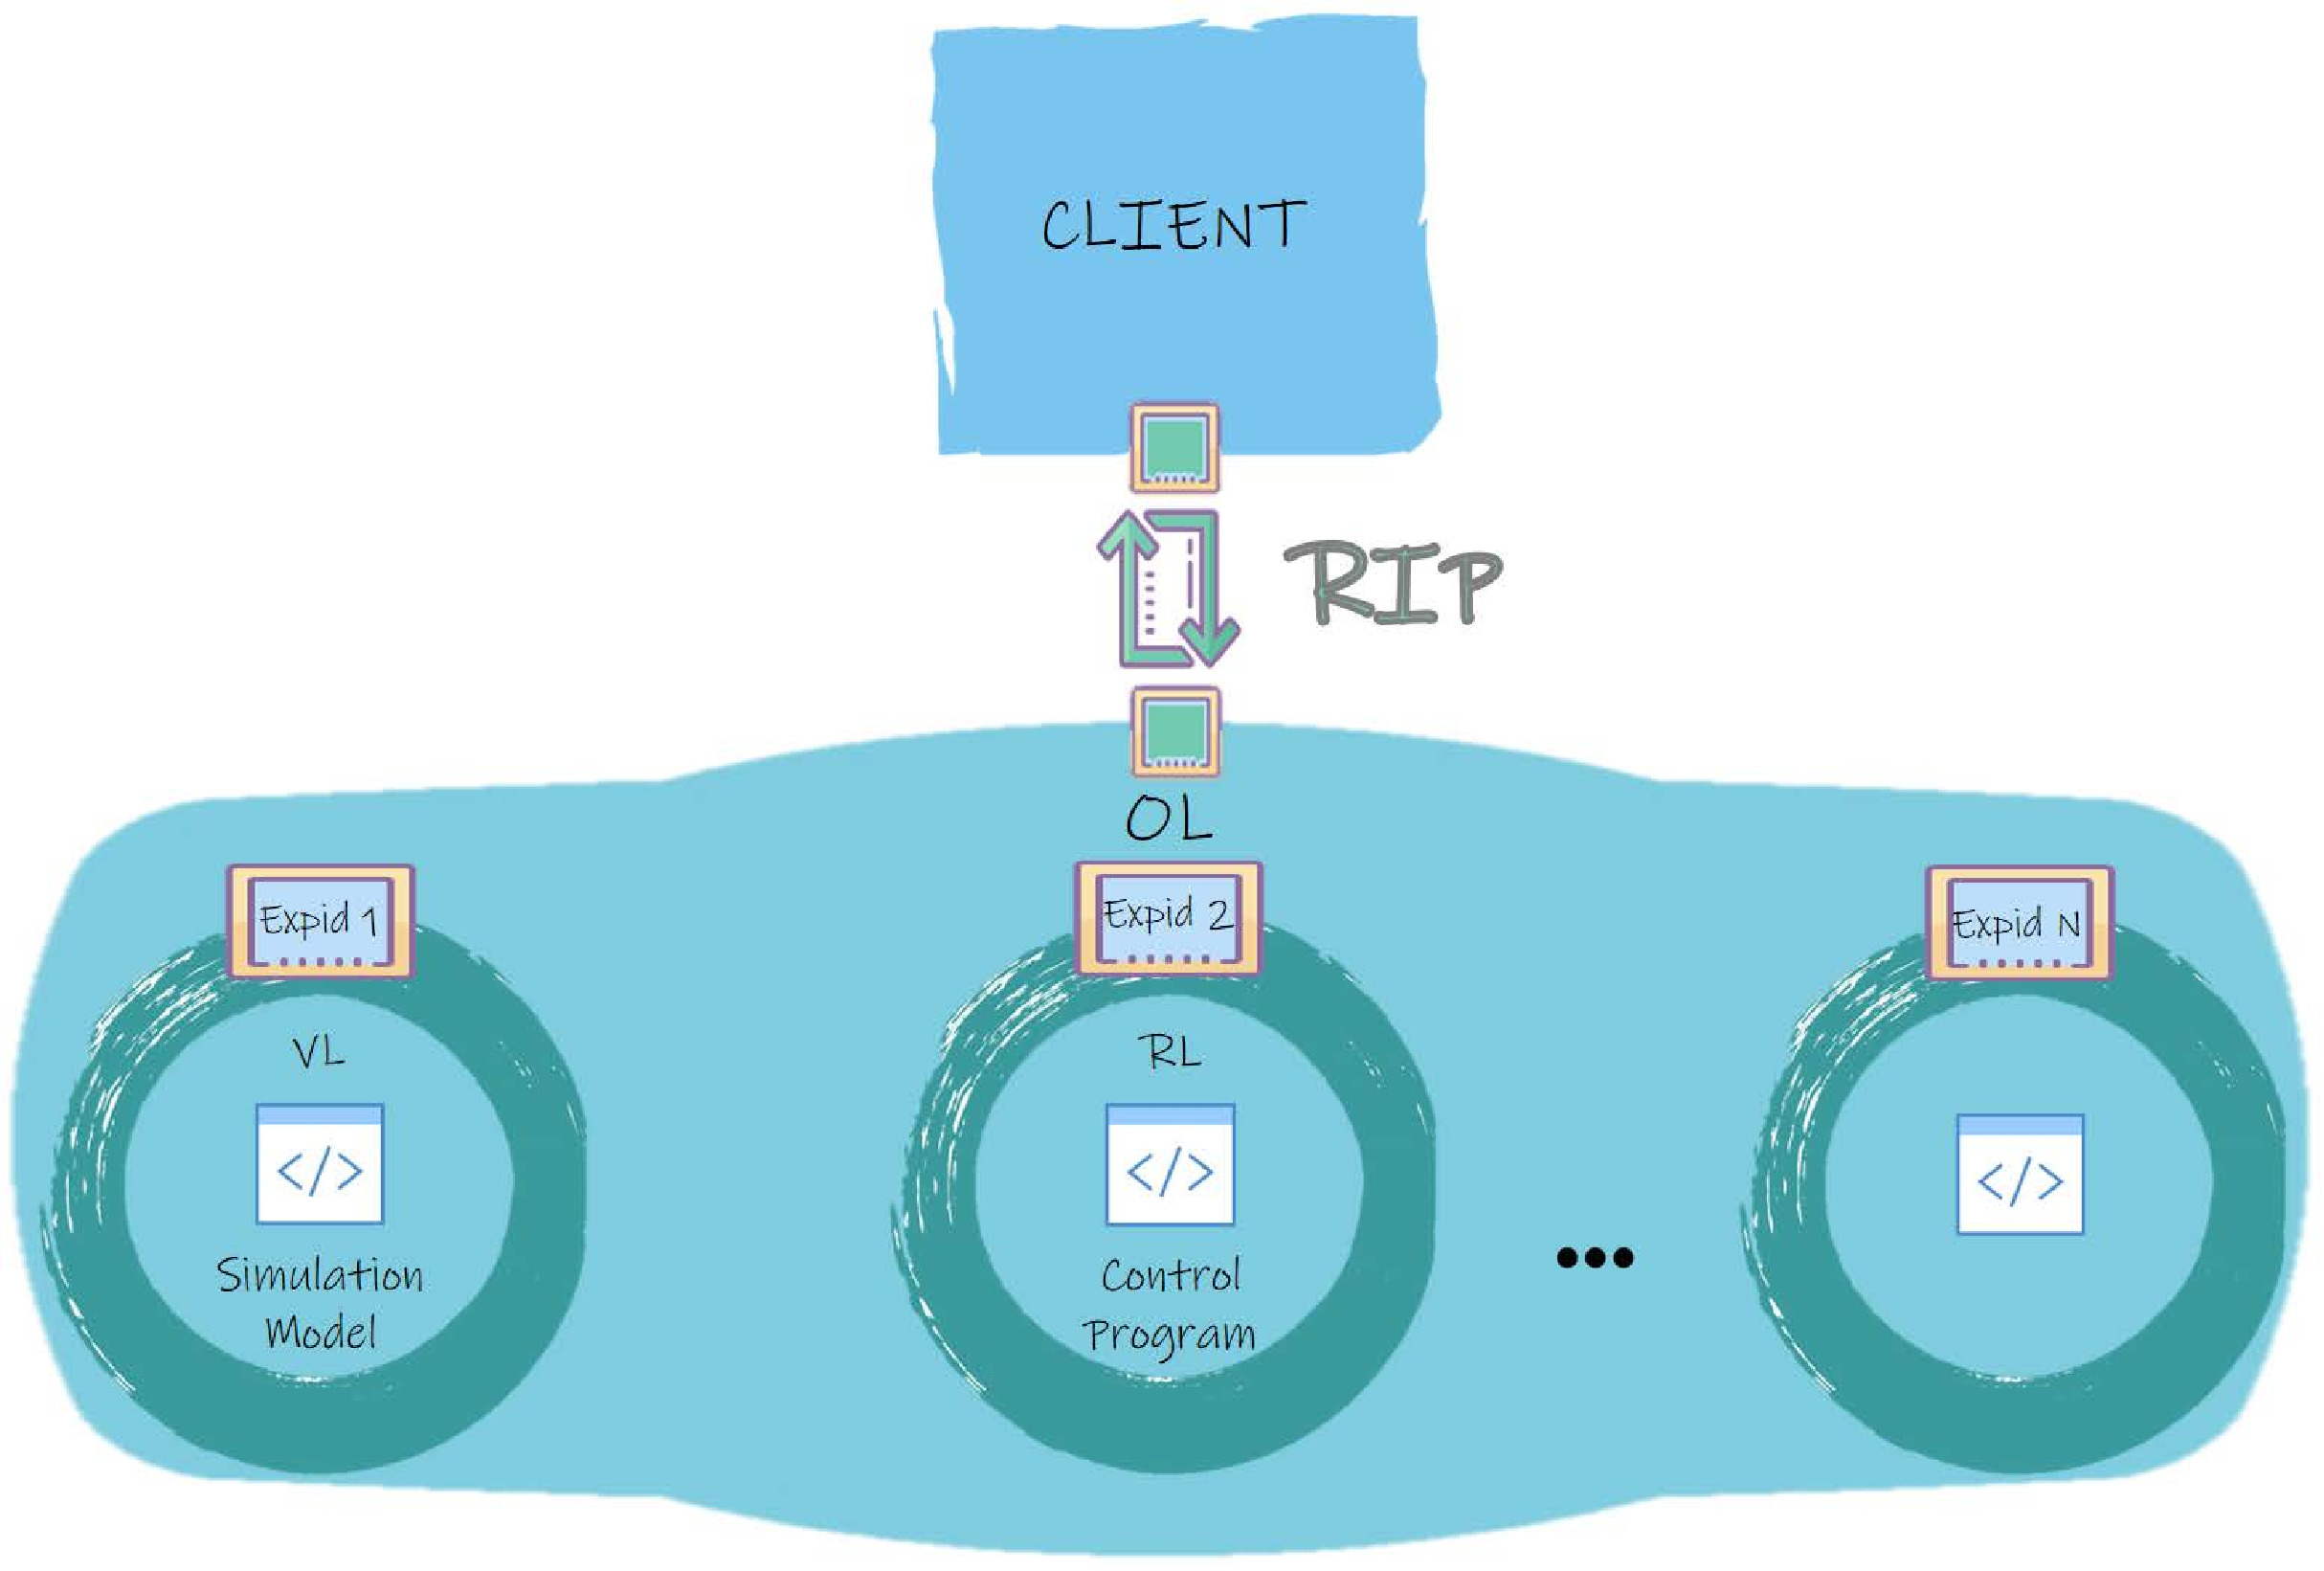
\includegraphics[width=0.75\textwidth]{images/Client-RIP-OL.pdf}
\caption{RIP Scope}
\label{fig:Client-RIP-OL}
\end{figure}


\chapter{Overall Description}
\label{Overall Description}

\section{Protocol Perspective}
The protocol is an open source, under the GNU general Public License. It is a communication protocol to be used in the client-server model, especially designed for OLs in which the client runs within a web browser. RIP provides a simple mechanism for users and client machines/programs to acquire information about the lab \textit{experiences} defined in the server and about each \textit{experience's} inputs and outputs. The protocol also defines mechanisms for reading and writing the values of these inputs and outputs, respectively.

The main features of RIP are the following:

\begin{enumerate}
    \item Defining \textit{experiences} on the OL.
    \item Obtaining meta-data related to each defined \textit{experience}.
    \item Obtaining a list of readable and writable variables for each \textit{experience}.
    \item Obtaining a list of methods to read and write variables in each \textit{experience}.
    \item Defining server events to send data either periodically or based on any other triggering condition defined in an \textit{experience}.
    \item Subscribing a client to any server event declared in an \textit{experience}.
\end{enumerate}

\subsection{Server Implementation Perspective}
Figure \ref{fig:RIP_Architecture} depicts the architecture of a \emph{RIP Server} that implements the RIP protocol. To sum it up, there are three functional subsystems: the \emph{Web Server}, that handles client connections, sessions, etc., the \emph{command interpreter}, that speaks the RIP protocol, and the \emph{executor}, that controls the execution of the laboratory \textit{control programs}.

\begin{figure}
\centering
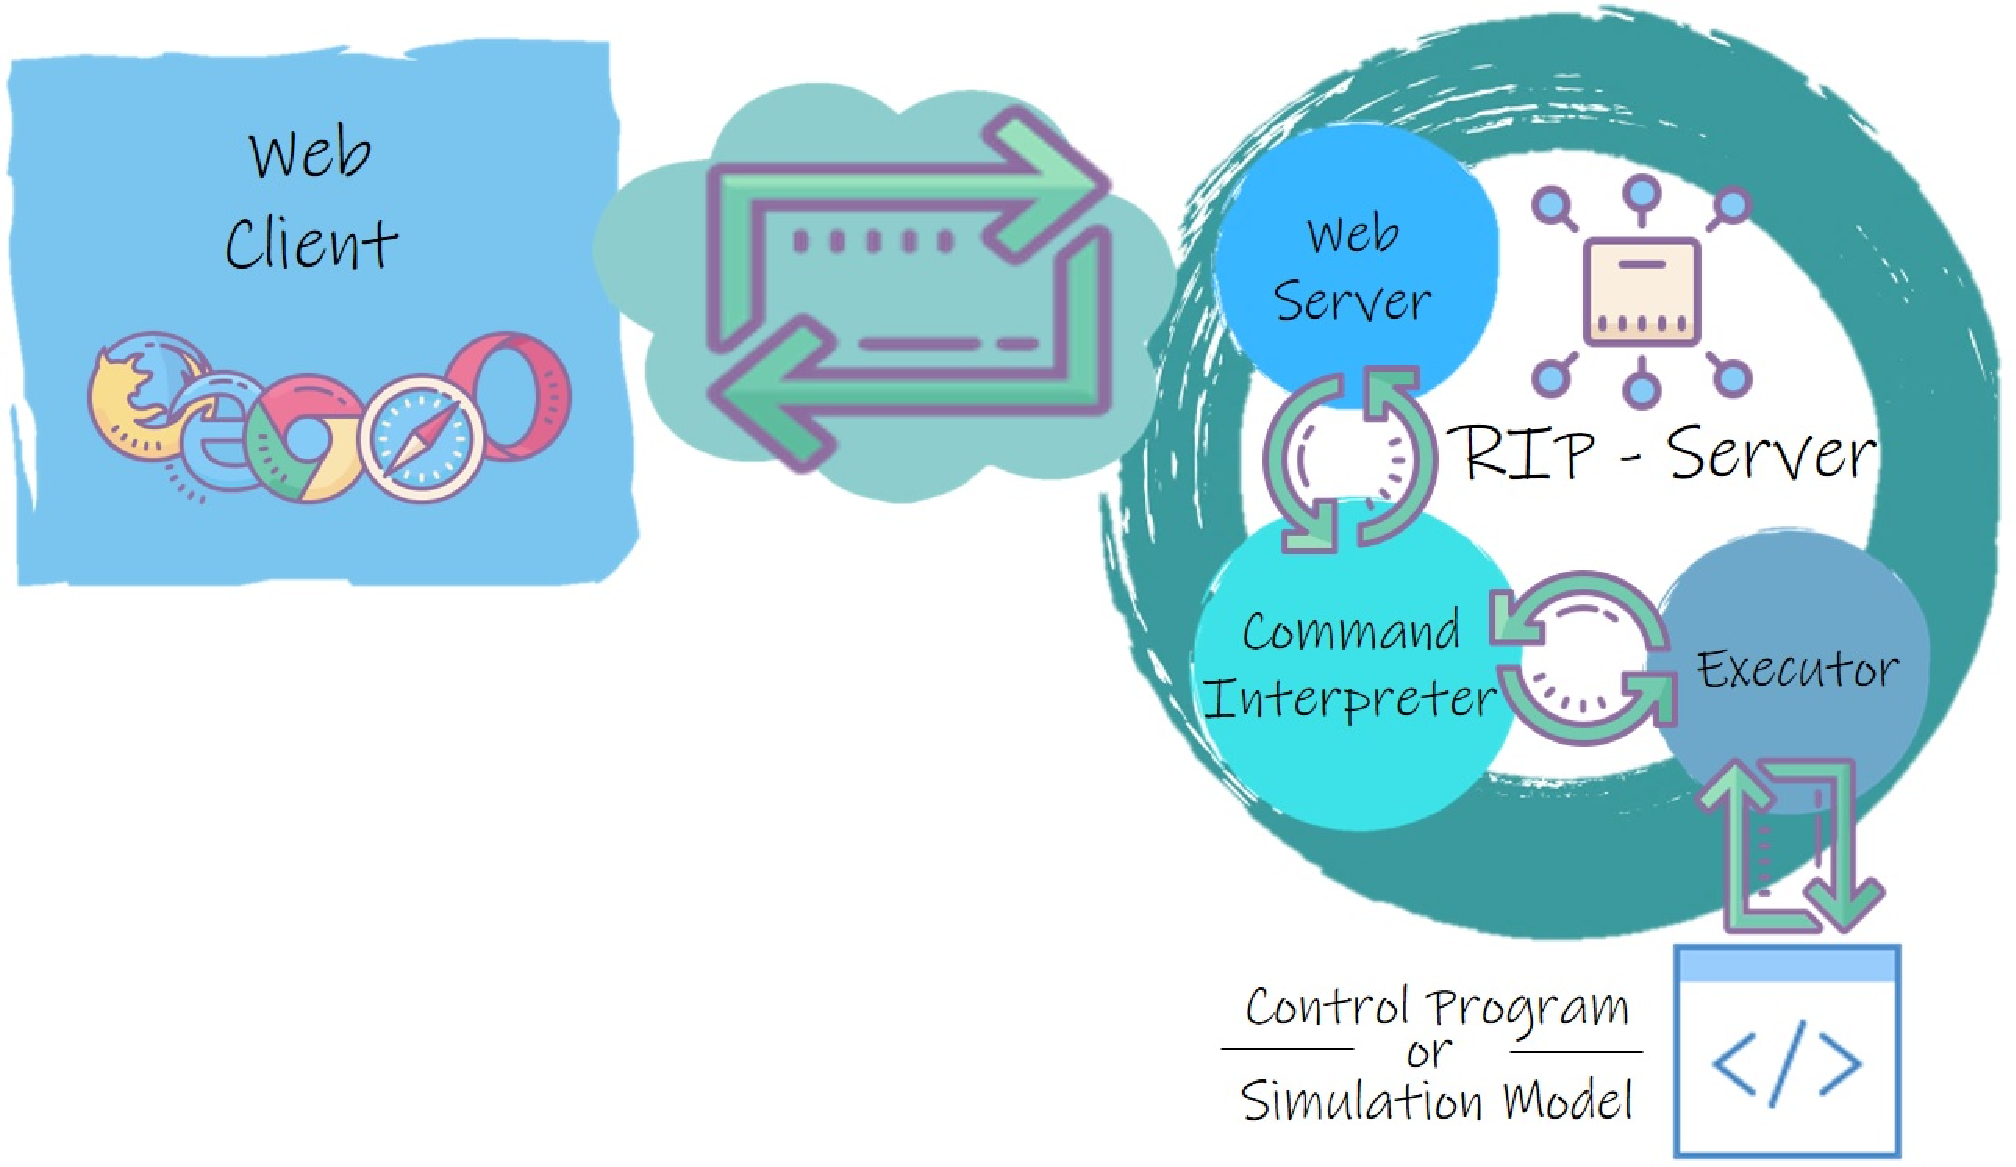
\includegraphics[width=0.75\textwidth]{images/RIPArchitecture.pdf}
\caption{Architectural view of a RIP Server}
\label{fig:RIP_Architecture}
\end{figure}

The Web Server admits (and handles in different ways) three types of requests: GET (used to retrieve \textit{experiences'} meta-data), SSE (used to get server-to-client data updates) and POST (used to send client-to-server updates). These different methods are each associated with the three basic cases of use, namely:

\begin{itemize}
    \item \emph{Meta-data} - A client, wanting to obtain information about the laboratory, launches an HTTP GET request to the URL associated with the laboratory. The laboratory responds with a JSON-RPC structure that informs the client, depending on the request's parameters, with one of the following:
    
    \begin{enumerate}
        \item General information about the OL: what are the \textit{experiences} defined and how they can be accessed.
        \item Detailed information of a particular \textit{experience} (when the request includes the {experience} id as a parameter).
    \end{enumerate}
    
    \item \emph{Observer} - A client, that desires to receive updates on the state of the plant, subscribes to an SSE event stream associated to the \textit{experience} of interest.
    
    \item \emph{Controller} - A client, wanting to act over the OL, sends a POST request with the command codified as a RIP-JSON-RPC structure.
\end{itemize}

An \textit{experience} represents a lab activity associated with an OL. In the case of RLs, each \textit{experience} is implemented as a \textit{control program}, which in general is responsible of managing the physical connections with the hardware, safe measures, and any other functionality the lab designer has considered appropriate to include. In the case of VLs, each \textit{experience} is implemented as a \textit{simulation model} that represents a real system. The \textit{experience} abstraction is useful for two purposes: 1) to publish information about OLs in a standard and structured way and 2) to allow for hosting and running several different \textit{control programs} or \textit{simulation models} in the same computer. 

\section{Protocol Functions}
The functions defined and used in the protocol are divided in two types: internal and external.

The internal functions are private functions, not exposed to the web clients. These methods are used internally by RIP server implementations to communicate either with the \textit{simulation model} or the \textit{control program} used in the OL.

The external functions are exposed through web services as public functions, and so, they are callable by the web clients. These methods are used by the clients to both get meta-data about the defined \textit{experiences} and to send and retrieve data to and from the OL.

\subsection{Internal Functions}
The list of existing internal functions a RIP server must implement is:

\begin{enumerate}
    \item \textit{readablelist}, \textit{writablelist}  = \textbf{open}(\textit{expid}): Returns the list of readable and writable variables (in two different variables) defined in the \textit{experience} associated to the input \textit{expid} parameter.
    \item \textbf{close}(\textit{expid}): Closes the control program (if it is a RL) or the simulation model (if it is a VL) of the OL \textit{experience} defined by the input \textit{expid} parameter.
\end{enumerate}

\subsection{External Functions}
The list of existing external functions a RIP server must implement so that a RIP client may use is:

\begin{enumerate}
    \item \textbf{info}(\textit{expid}): Retrieves the meta-data information about the \textit{experience} defined by the input \textit{expid} parameter. 
    \item \textbf{start}(\textit{expid}): Starts the execution of the control program (if it is a RL) or the simulation model (if it is a VL) of the OL \textit{experience} associated to the input \textit{expid} parameter.
    \item \textbf{stop}(\textit{expid}): Stops the execution of the control program (if it is a RL) or the simulation model (if it is a VL) of the OL \textit{experience} defined by the input \textit{expid} parameter.
    \item \textit{readvariablenames}, \textit{readvariablevalues} = \textbf{get}(\textit{expid}, \textit{variablenames}): Retrieves the current values of the variables (\textit{readvariablevalues}) specified by the \textit{variablenames} input parameter. For this to happen, these variables must exist in the \textit{control program} or \textit{simulation model} associated to the \textit{experience} defined by the \textit{expid} input parameter. When the \textbf{get()} method is called, \textit{readvariablenames} contains only the names of the variables that were successfully read, not all requested ones in \textit{variablenamess}.
    \item \textbf{set}(\textit{expid}, \textit{variablenames}, \textit{variablevalues}): Writes the received values (\textit{variablevalues}) in the specified variables (\textit{variablenames}) of the appropiate OL \textit{experience}. For this to happen, these variables must exist in the \textit{control program} or \textit{simulation model} associated to the (\textit{expid}) input parameter.
\end{enumerate}

Where:

Variables \textit{variablenames} and \textit{variablevalues} are arrays of text. For example: \textit{variablenamess} = ["x", "y", ...], \textit{variablevalues} = ["10", "a", ...].

Each method returns an error indicator when the operation is not completed successfully.

At the moment, only numbers, text and booleans are supported in the \textbf{set}() and \textbf{get}() methods.

\section{Operating Environment}
RIP uses only HTTP methods for the communication. Therefore, it works in any major web browser. However, RIP also relies on the use of SSE, which, up to date, are not supported by Microsoft Internet Explorer nor Microsoft Edge. Nevertheless, there are numerous poly-fill solutions for implementing SSE so that they work on these browsers that do not support them natively.

\section{Design and Implementation Constraints}
RIP is designed to only use pure HTTP methods on purpose, with the aim of guaranteeing its correct functioning from web browsers.

\section{Assumptions and Dependencies}
RIP depends solely on the use of HTTP POST and GET methods and on the JSON format for exchanging data.

\section{User Documentation}
TODO


\chapter{External Interface Requirements}
\label{External Interface Requirements}

\section{User Interfaces}
TODO

\section{Software Interfaces}
TODO

\section{Communications Interfaces}
TODO


\chapter{Protocol Features}
\label{System Features}

\section{Defining Experiences}
TODO

\section{Obtaining Meta-data}
TODO

\section{Obtaining Readable and Writable Variables}
TODO

\section{Obtaining and Calling Interface Methods}
TODO

\section{Defining Server Events}
TODO

\section{Subscribing to Server Events}
TODO


\begin{appendices}

\chapter{Glossary}
\textbf{Control program -} A software program which purpose is to control and monitor the hardware equipment used to in a laboratory activity.

\textbf{Experience -} Any lab activity that can be performed in an OL.

\textbf{OL -} Online laboratory.

\textbf{RIP -} Remote Interoperability Protocol.

\textbf{RL -} Remote laboratory.

\textbf{Simulation model -} A mathematical simulation that models a certain system with which laboratory activities can be carried out.

\textbf{SSE -} Server-sent events.

\textbf{VL -} Virtual laboratory.


\chapter{Analysis Models}
TODO

\end{appendices}

\bibliographystyle{alpha}
\renewcommand\bibname{References}
\bibliography{base/sources}